\graphicspath{{results/fig/}}

\chapter{Results}

\section{Data logging}
The resulting GPS coordinates that were stored to the micro-SD card during the data logging test were plotted on a map of Stellenbosch, and are shown in red in Fig.\ref{fig:rooi-plane-loop}.
The actual path that was travelled was a loop starting on the corner of Victoria and Ryneveld street, then a left turn onto Bosman street, a left turn onto Merriman avenue and 
a left turn back onto Ryneveld street. 

\begin{figure}[!h]
    \centering
    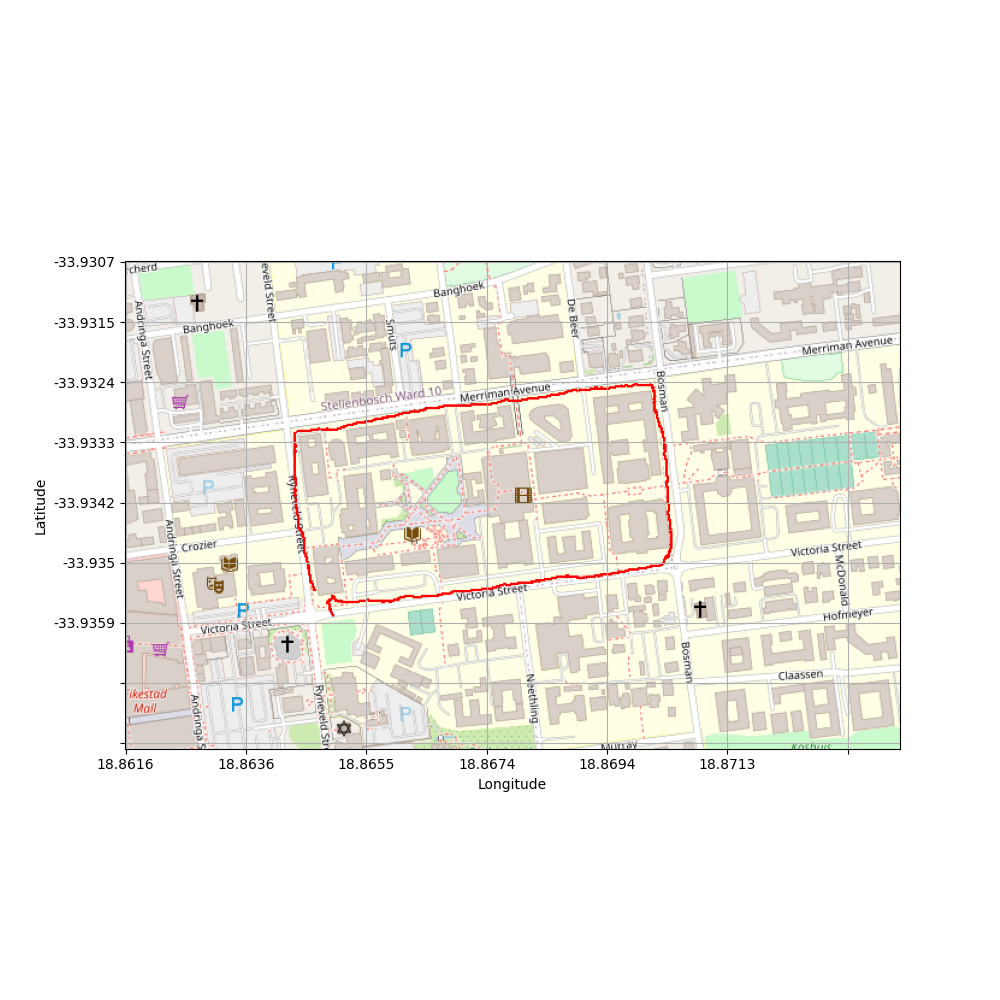
\includegraphics[width=0.8\linewidth]{rooi_plane_loop.png}
    \caption[Data logging test]{GPS coordinates of path travelled}
    \label{fig:rooi-plane-loop}
\end{figure}

The GPS coordinates correspond approximately to the actual path that was travelled, and the accuracy of the GPS receiver is therefore sufficient for the purposes of this project. These results 
have also verified the data logging capabilities of the system. 

\section{Digital Compass}
Two separate tests where done to test the accuracy of the digital compass. The results of the first test are shown in Fig.\ref{fig:digital-compass-test-1}. The error between the digital compass
and the handheld compass is shown in Fig.\ref{fig:digital-compass-test-1-error}. The average error was calculated to be $6.7312^{\circ}$. The error can be attributed to a inadequate calibration
process - compass rotation does not cover all possible angles, calibration process too short or sample frequency used not high enough.

\begin{figure}[!h]
    \centering
    \begin{subfigure}[!h]{=0.9\linewidth}
        \centering
        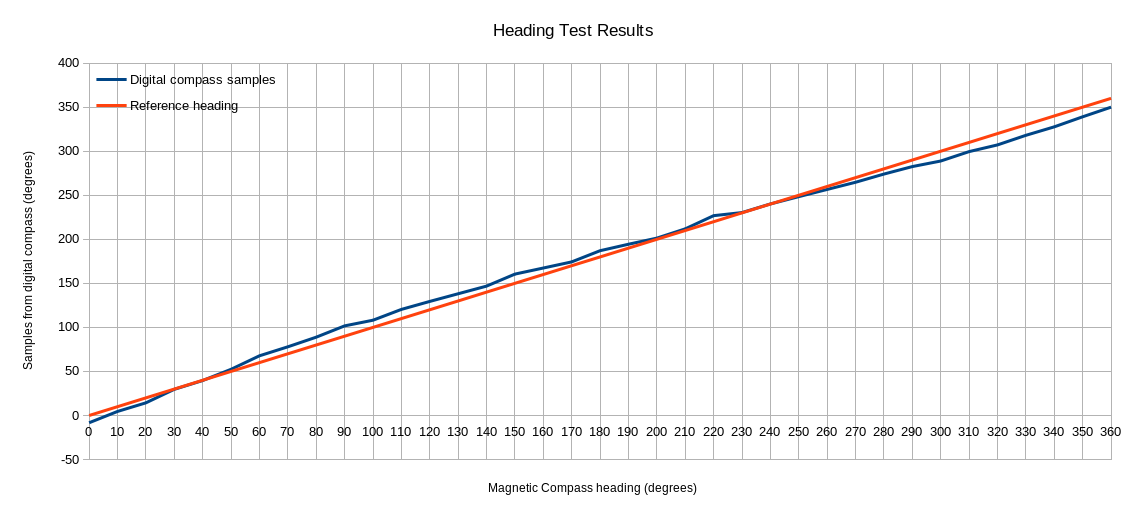
\includegraphics[width=1\linewidth]{digital-compass-test-1.png}
        \caption{Digital compass heading compared to handheld compass heading}
        \label{subfig:digital-compass-test-1}
    \end{subfigure}

    \begin{subfigure}[!h]{=0.9\linewidth}
        \centering
        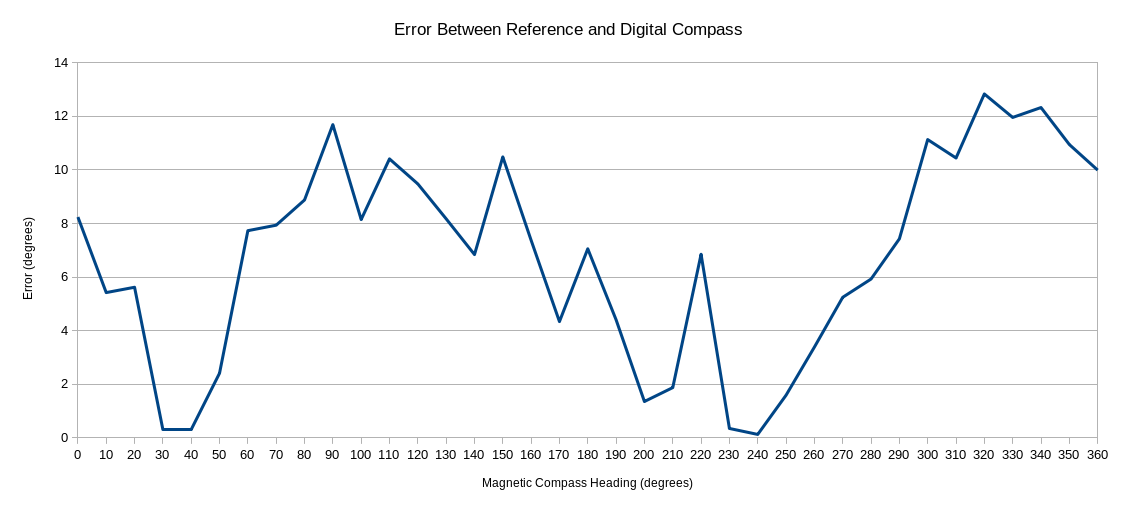
\includegraphics[width=1\linewidth]{digital-compass-test-1-error.png}
        \caption{Error between Digital compass heading and handheld compass heading}
        \label{subfig:digital-compass-test-1-error}
    \end{subfigure}
    \caption[Digital compass accuracy test-1]{Digital compass accuracy test}
    \label{fig:Digital compass accuracy test-1}
\end{figure}

The test was therefore redone, this time an extensive calibration of the digital compass was done. The results of the second test are shown in Fig.\ref{subfig:digital-compass-test-2}. The error 
between the digital compass and the handheld compass is shown if Fig.\ref{subfig:digital-compass-test-2-error}. The average error for this test was calculated as $1.5091^{\circ}$. The results of
this test verify that the digital compass is accurate when placed on a flat surface.

\begin{figure}[!h]
    \centering
    \begin{subfigure}[!h]{=0.9\linewidth}
        \centering
        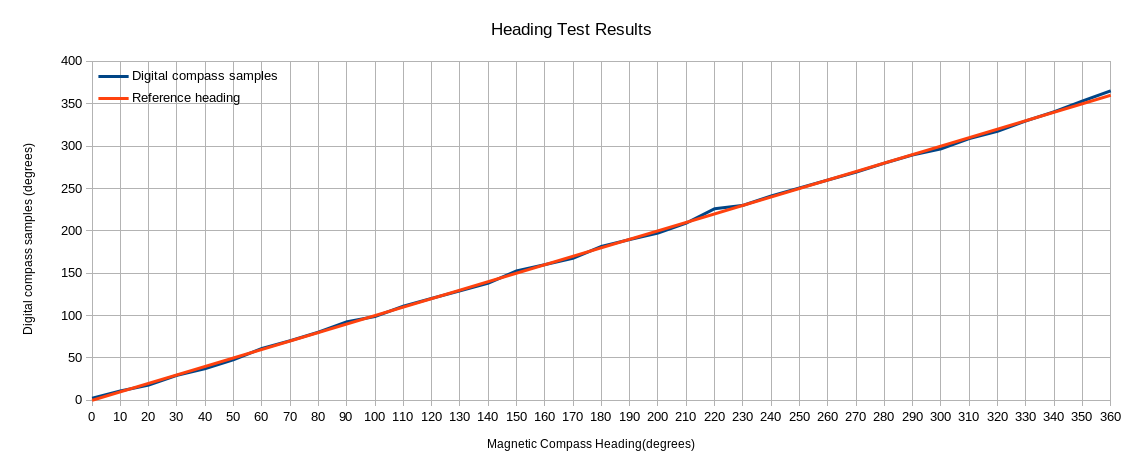
\includegraphics[width=1\linewidth]{digital-compass-test-2.png}
        \caption{Digital compass heading compared to handheld compass heading}
        \label{subfig:digital-compass-test-2}
    \end{subfigure}

    \begin{subfigure}[!h]{=0.9\linewidth}
        \centering
        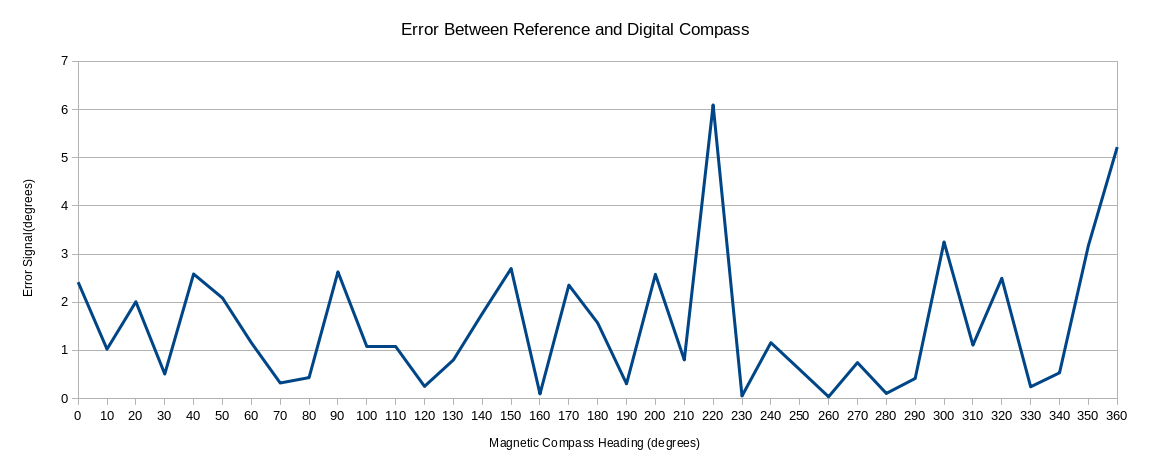
\includegraphics[width=1\linewidth]{digital-compass-test-2-error.png}
        \caption{Error between Digital compass heading and handheld compass heading}
        \label{subfig:digital-compass-test-2-error}
    \end{subfigure}
    \caption[Digital compass accuracy test-2]{Digital compass accuracy test}
    \label{fig:Digital compass accuracy test-2}
\end{figure}

The results of the tilt compensation test are shown in Fig.\ref{subfig:tilt-comp-error}. It should be noted that this test was conducted using the same calibration values (hard-iron offset and 
soft-iron correction values) that were determined and used in Fig.\ref{fig:Digital compass accuracy test-1}. The results of the tilt compensation test are therefore compared to the results of 
the test done in Fig.\ref{fig:Digital compass accuracy test-1}. 

\begin{figure}[!h]
    \centering
    \begin{subfigure}[!h]{=0.9\linewidth}
        \centering
        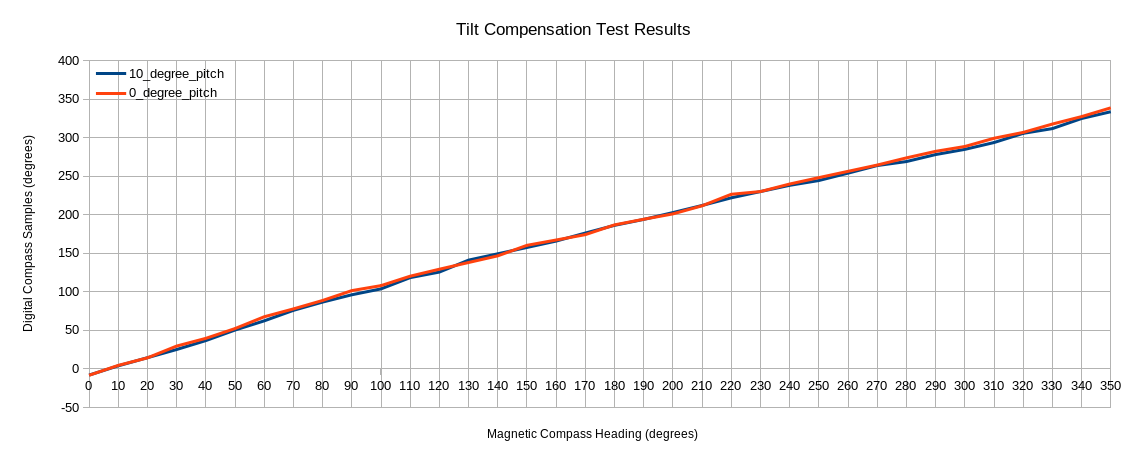
\includegraphics[width=1\linewidth]{tilt-comp-test.png}
        \caption{Tilt compensated digital compass heading compared to handheld compass heading}
        \label{subfig:tilt-comp-test}
    \end{subfigure}

    \begin{subfigure}[!h]{=0.9\linewidth}
        \centering
        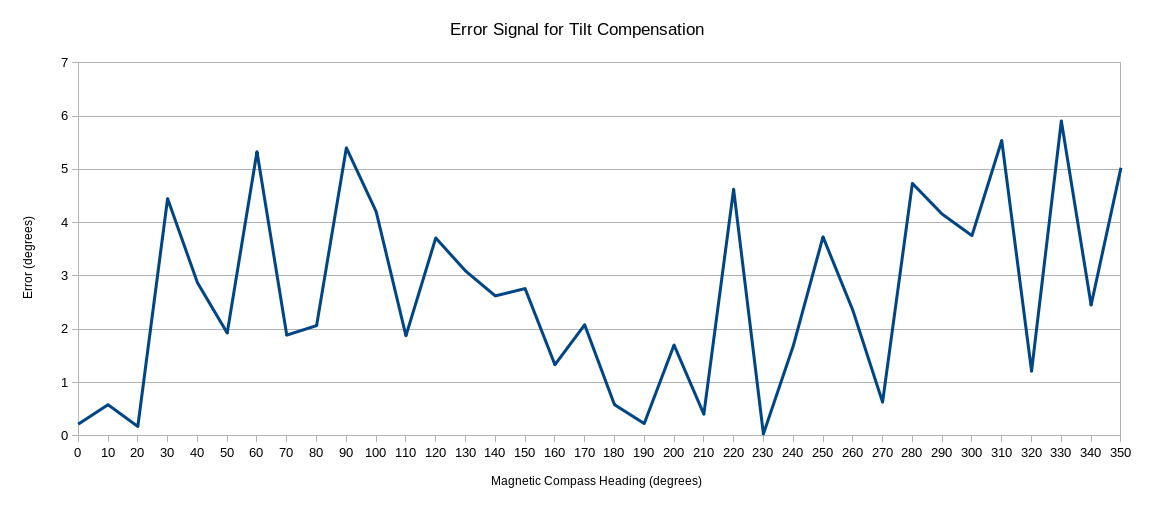
\includegraphics[width=1\linewidth]{tilt-comp-test-error.png}
        \caption{Error between tilt compensated digital compass heading and handheld compass heading}
        \label{subfig:tilt-comp-error}
    \end{subfigure}
    \caption[Tilt compensation test]{Tilt compensation algorithm test}
    \label{fig:tilt-comp}
\end{figure}

The tilt-compensated digital compass readings are approximately equal to the results obtained when the digital compass had a pitch angle of zero. The error in the results seen in Fig.\ref{subfig:tilt-comp-error}
can be attributed to the slight difference in angle when adjusting the wooden platform by hand between the $10^{\circ}$ steps. The average error was found to be equal to $2.6502^{\circ}$. The calculations done
in section \ref{sec: ...} show that the samples taken at varying degrees of pitch angle should theoretically be the same. The results shown in Fig.\ref{fig:tilt-comp} show that the tilt compensation 
algorithm does work.

\section{Sail Control}
\label{sail-control}

The first test was done to verify the accuracy of the wind direction measurements, the results are shown in Fig.\ref{subfig:wind-test}. From these results it can be seen that the measured wind 
direction deviates slightly from the actual direction of the wind vain. The purpose of the wind sensor is to determine the optimal sail position, sail position does not however affect the navigation
of the vessel, only the speed of the vessel. Therefore absolute accuracy in measuring wind direction is not of the utmost importance, and deviation in measured results is acceptable.

\begin{figure}
    \centering
    \begin{subfigure}[h!]{0.49\textwidth}
      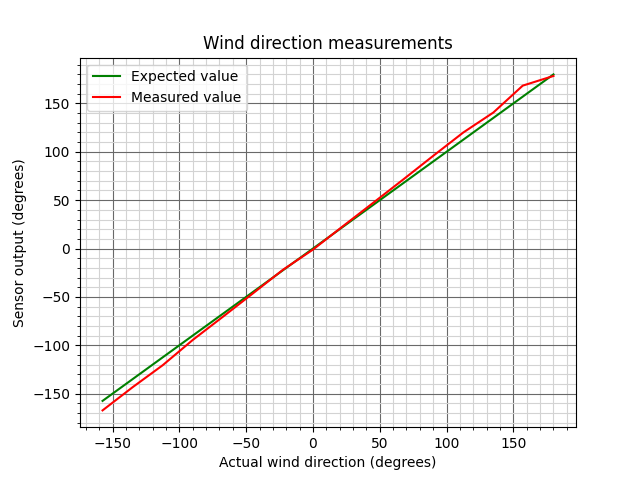
\includegraphics[width=\textwidth]{sail-control/sensor-output.png}
      \caption{Actual and measured wind direction}
      \label{fig:wind-test}
    \end{subfigure}
    %
    \begin{subfigure}[h!]{0.49\textwidth}
      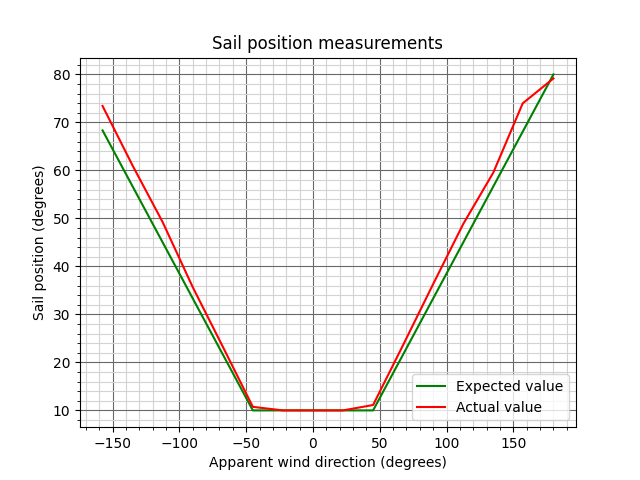
\includegraphics[width=\textwidth]{sail-control/sail-pos.png}
      \caption{Measured and expected sail position}
      \label{fig:sail-pos-test}
    \end{subfigure}
    \caption[Sail controller test results]{Sail controller test results}
    \label{fig:sail-control}
\end{figure}

The second test conducted, measured the change in sail position given a change in apparent wind direction. The 
results of this test are shown in Fig.\ref{subfig:sail-control}. The resulting measurements closely match the expected results. The sail position is at approximately $80^{\circ}$ when the apparent 
wind is at $\pm 180^{\circ}$, sail position then decreases linearly as the absolute apparent wind value decreases towards $45^{\circ}$ - limit of no-sail zone - which corresponds to a sail position 
of $10^{\circ}$. As expected the sail position stays at $10^{\circ}$ for apparent wind in the range $\pm 45^{\circ}$. 


\section{Rudder control}
\subsection{Test-1}
\label{test-1}

The results of the rudder control test which was conducted out of the water are shown in Fig.\ref{fig:rudder-control-dry}. The average value of reference heading is $44.603^{\circ}$ and the average value of actual 
heading is $44.728^{\circ}$. These values are approximately equal and therefore the error signal that is generated for the rudder controller should keep the vessel on course when on water. The variance of the 
actual heading during the test was calculated as $13.178^{\circ}$, which can be attributed to slight sway when walking.  

\begin{figure}[h!]
    \centering
    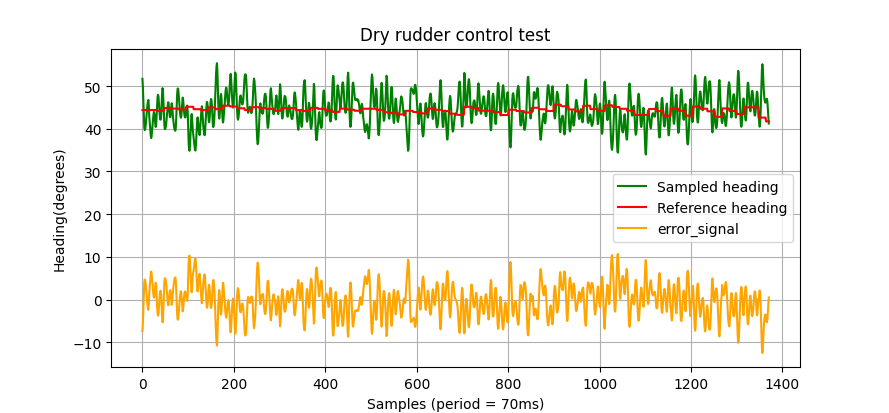
\includegraphics[width=1\linewidth]{dry-rudder-test.png}
    \caption[Rudder control test out of water]{Results of rudder control test out of water}
    \label{fig:rudder-control-dry}
\end{figure}

% For the first rudder control test conducted on the water, the apparent wind was determined before hand to be roughly $100^{\circ}$, the sail position was therefore set to $40^{\circ}$.%NB must work this out using updates sail position formulae i.e. one with new pwm_min value 
% The target coordinate given to the system corresponded to a location on the side of the dam. The proportional gain factor was set to 1.5 and integral gain factor was set to zero. The GPS 
% coordinates logged during the test were plotted with Python and are shown in Fig.\ref{fig:rudder-control-test-1-path}. 

\subsection{Test-2}
\label{test-2}

For the first rudder control test conducted on the water, the apparent wind was determined before hand to be roughly $100^{\circ}$, the sail position was therefore set to $40^{\circ}$.%NB must work this out using updates sail position formulae i.e. one with new pwm_min value 
For this test instead of calculating the reference heading - using the current GPS coordinates and target GPS coordinates - on every iteration a fixed reference bearing was set as $113^{\circ}$ 
beforehand. The proportional gain factor was set to 1.8. The GPS coordinates logged during the test were plotted with Python and are shown in Fig.\ref{fig:rudder-control-test-1-path}. 

%Actual value during this test was 1.5

\begin{figure}[h!]
    \centering
    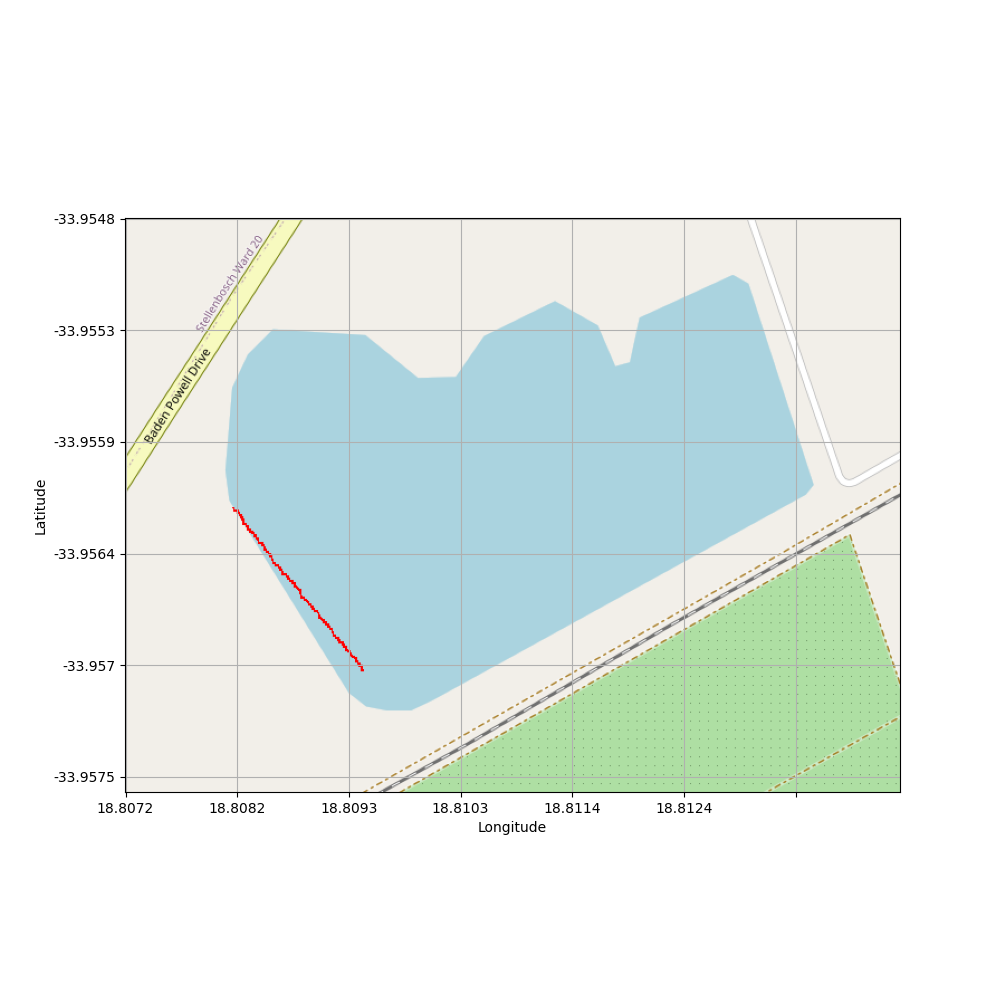
\includegraphics[width=0.8\linewidth]{dam-test-1/dam-test-1.png}
    \caption[Path travelled in first rudder control test]{GPS coordinates of path travelled}
    \label{fig:rudder-control-test-1-path}
\end{figure}

 
During the test the vessel was visibly oscillating from starboard to port side, this can be seen when analyzing Fig.\ref{subfig:first-rudder-control-heading}, which is a plot of the measured 
heading and reference heading data, logged throughout the test. The average actual heading value is $115,404^{\circ}$ and the variance is $216,495^{\circ}$. The oscillation indicates that 
the proportional gain factor is too high and overshoot is occurring. 

\begin{figure}[h!]
    \centering
    \begin{subfigure}{=0.75\linewidth}
        \centering
        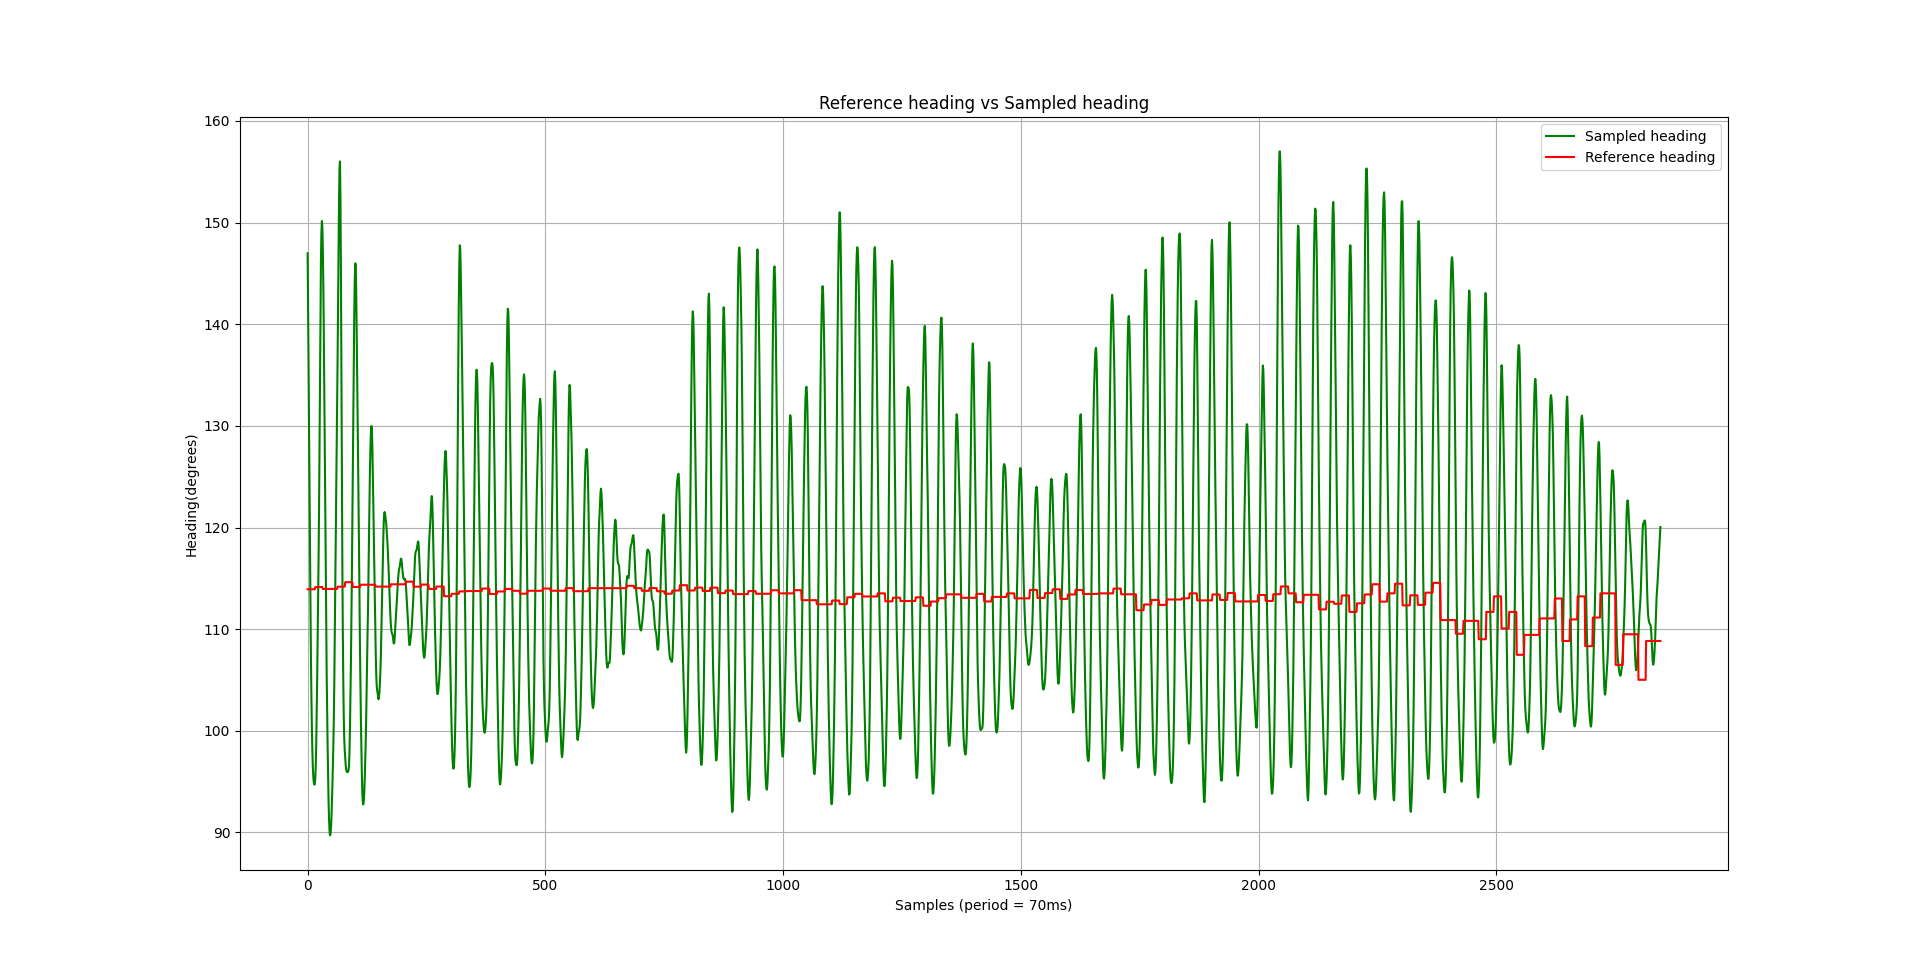
\includegraphics[width=1\linewidth]{dam-test-1/heading.png}
        \caption{sampled and reference heading}
        \label{subfig:first-rudder-control-heading}
    \end{subfigure}

    \begin{subfigure}{=0.75\linewidth}
        \centering
        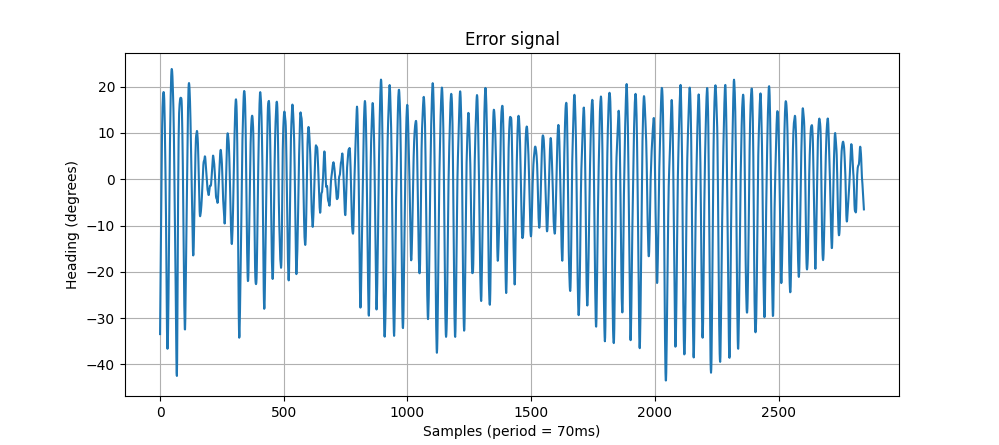
\includegraphics[width=1\linewidth]{dam-test-1/error.png}
        \caption{Error signal}
        \label{subfig:first-rudder-control-error}
    \end{subfigure}

    \begin{subfigure}{=0.75\linewidth}
        \centering
        \includegraphics[width=1\linewidth]{dam-test-1/wind.png}
        \caption{Apparent wind}
        \label{subfig:first-rudder-control-wind}
    \end{subfigure}

    \caption[First rudder control test on water]{First rudder control test on water}
    \label{fig:first-rudder-control-water}
\end{figure}


The error signal, which is input to the rudder 
controller is shown in Fig.\ref{subfig:first-rudder-control-error}. The maximum speed reached during the test was 1.161 knots. Although the sail controller was not implemented during this test, 
wind direction readings were still taken and the data is illustrated in Fig.\ref{subfig:first-rudder-control-wind}. The average apparent wind value is $98.8^{\circ}$, which corresponds to the initial 
wind direction reading that was taken. The variation in apparent wind direction throughout the test can be attributed to the oscillating of the vessel.

\subsection{Test-3}
\label{test-3}
%Put successful straight line test here
Another test was conducted on the water, this time the reference heading was calculated using current and target GPS coordinates after every sampling period. A GPS coordinate corresponding to a 
point on the side of the dam was set as the target location. The proportional gain factor was set to 1.4. The sail position controller was again not used during this test, instead the apparent wind
was measured beforehand. The apparent wind direction was determined to be $-85^{\circ}$ and the sail position was set to $40^{\circ}$. The GPS coordinates that were logged throughout the test 
are shown in Fig.\ref{fig:rudder-control-test-2-path}.

\begin{figure}[h!]
    \centering
    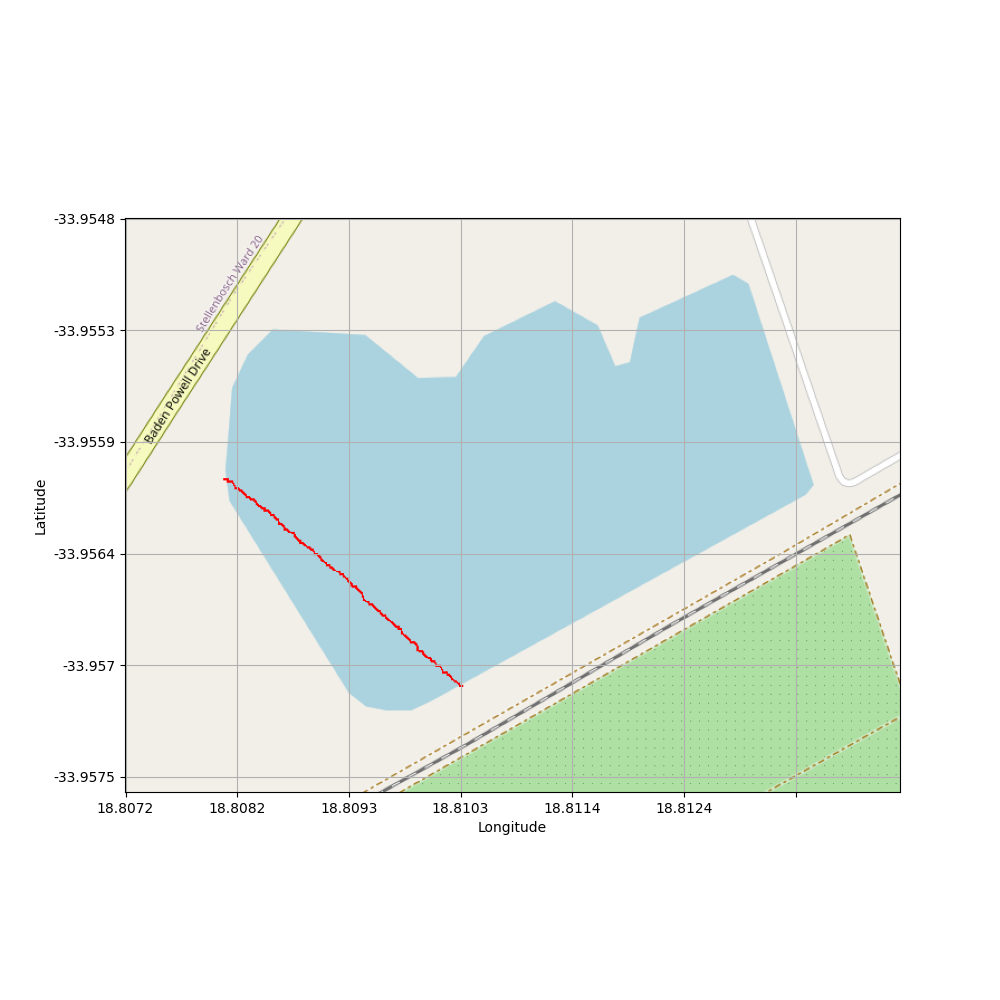
\includegraphics[width=0.8\linewidth]{dam-test-2/dam-test-3.png}
    \caption[Path travelled in first rudder control test]{GPS coordinates of path travelled}
    \label{fig:rudder-control-test-2-path}
\end{figure}

The reference and actual bearing values that were logged throughout the test are shown in Fig.\ref{subfig:rudder-contorl-2-heading}. The error signal that was generated for the rudder controller 
can be seen in Fig.\ref{subfig:rudder-control-2-error}. The average of the actual bearing is $112.32^{\circ}$ and the variance is $4.77^{\circ}$. The average of the reference heading is
$111.26^{\circ}$. The variance of the actual bearing is similar to that of Test-1, the proportional gain value of 1.4 is therefore close to optimal. The difference between the actual and reference 
heading averages is very slight and the rudder controller therefore tracked the reference signal sufficiently.

\begin{figure}[h!]
    \centering
    \begin{subfigure}{=0.75\linewidth}
        \centering
        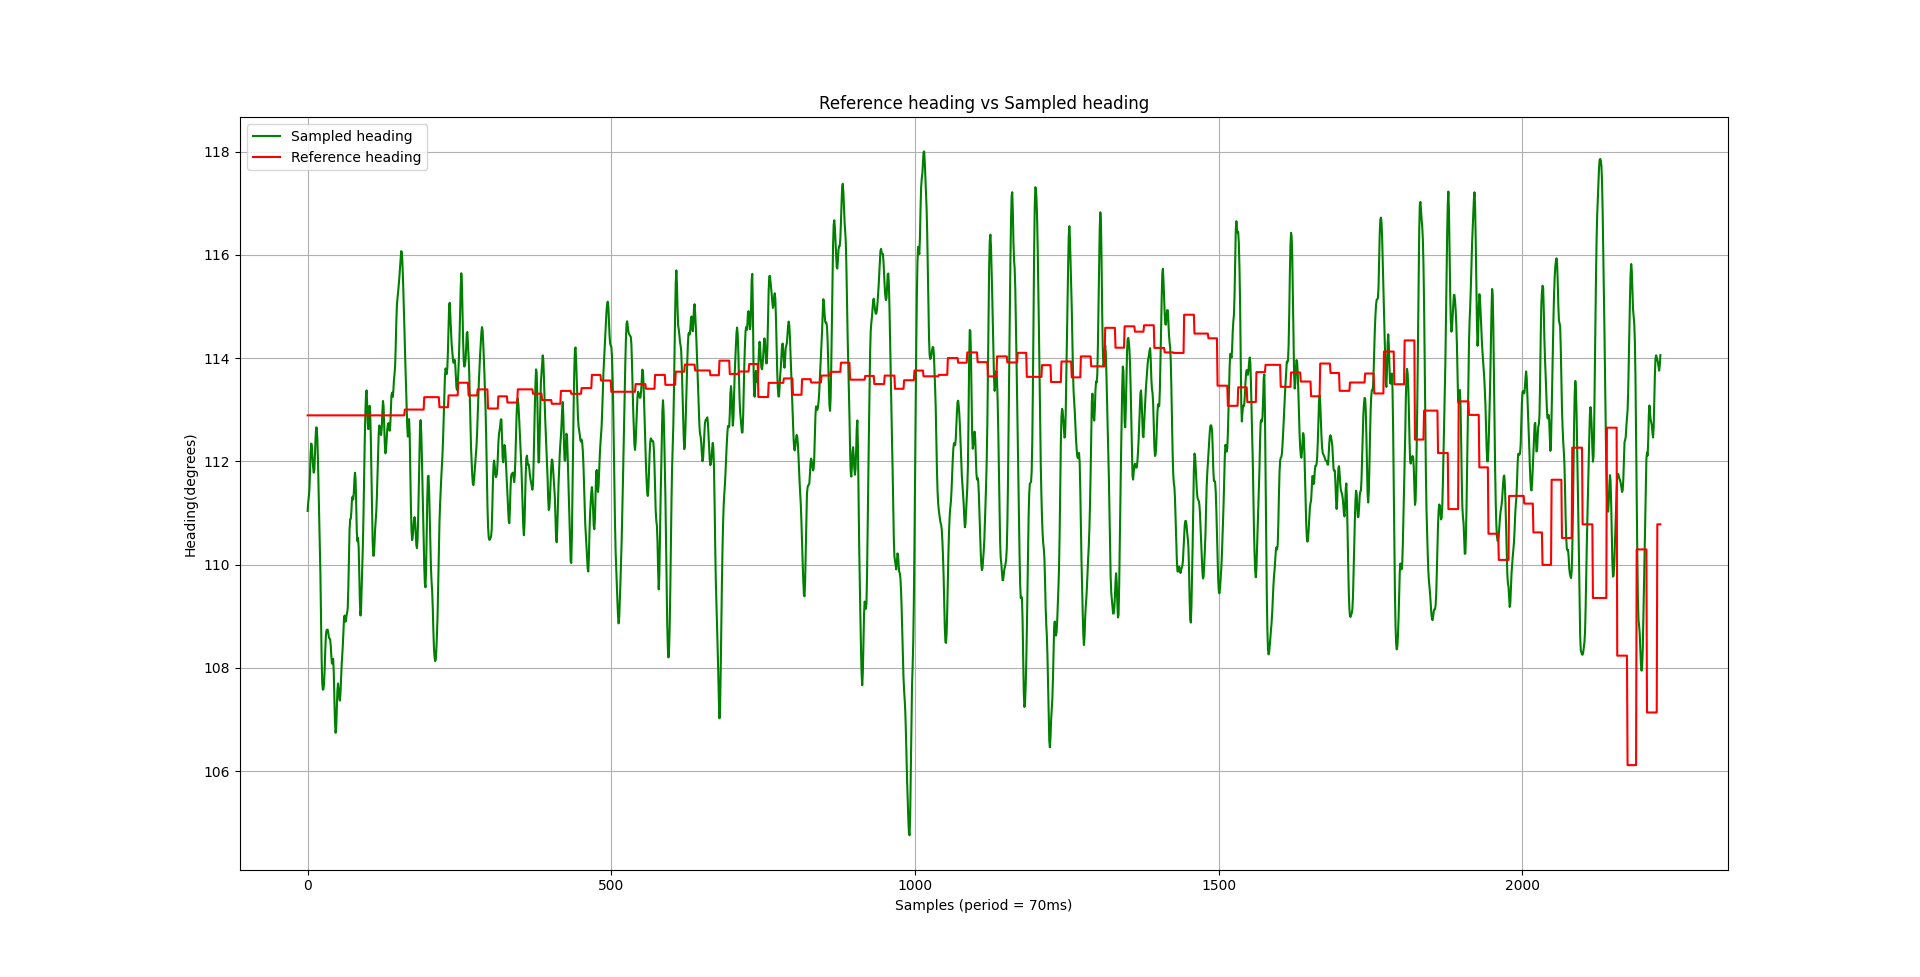
\includegraphics[width=1\linewidth]{dam-test-2/heading-graph.png}
        \caption{sampled and reference heading}
        \label{subfig:rudder-control-2-heading}
    \end{subfigure}

    \begin{subfigure}{=0.75\linewidth}
        \centering
        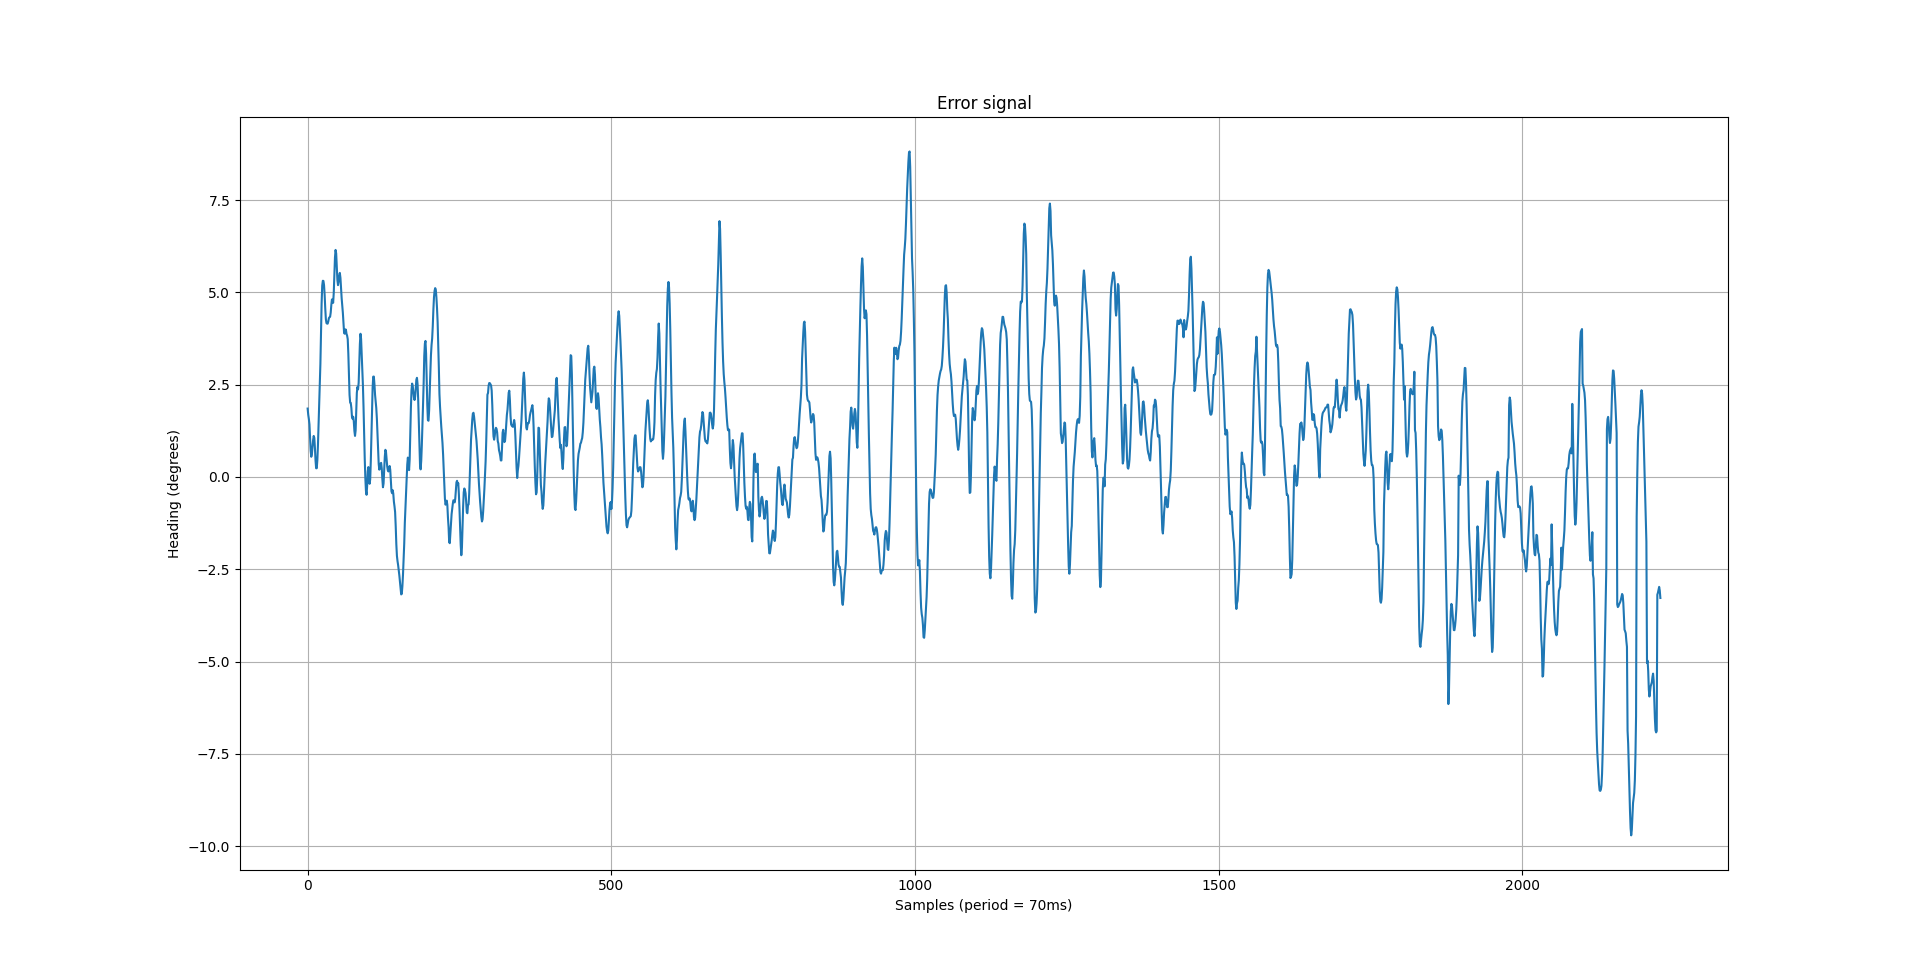
\includegraphics[width=1\linewidth]{dam-test-2/error-graph.png}
        \caption{Error signal}
        \label{subfig:rudder-control-2-error}
    \end{subfigure}

    \begin{subfigure}{=0.75\linewidth}
        \centering
        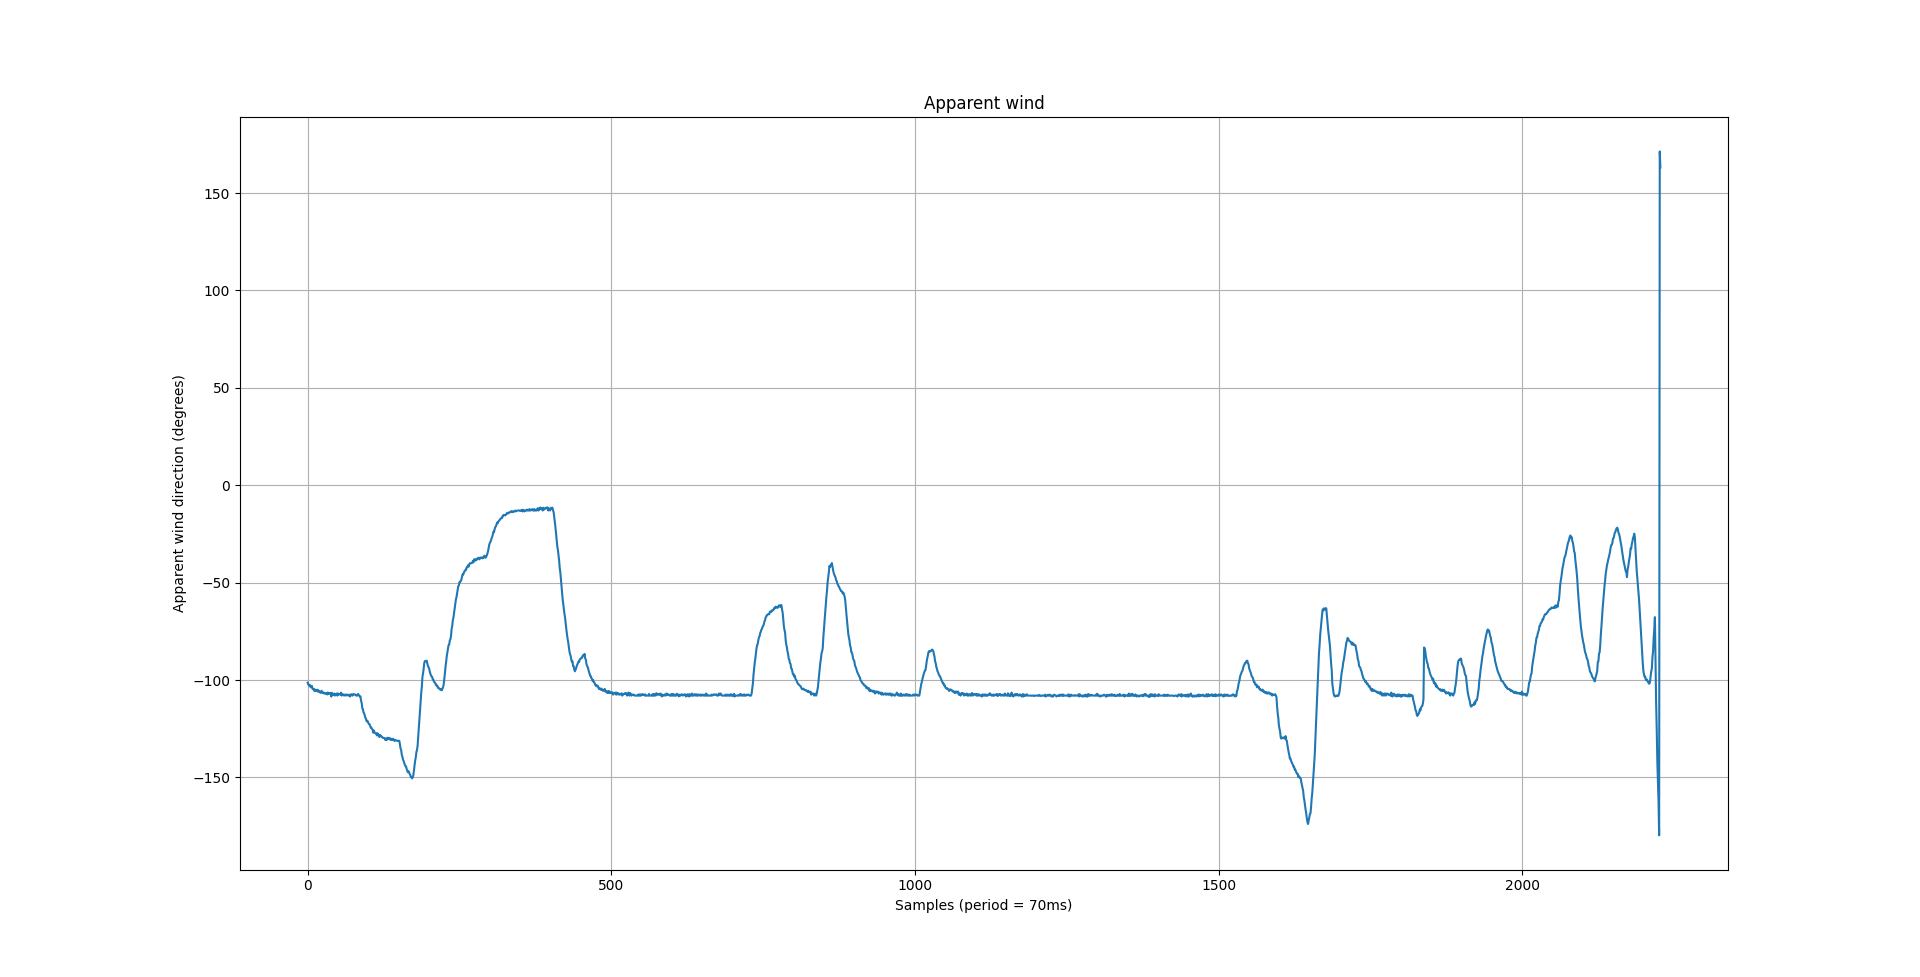
\includegraphics[width=1\linewidth]{dam-test-2/apparent-wind.png}
        \caption{Apparent wind}
        \label{subfig:rudder-control-2-wind}
    \end{subfigure}

    \caption[Second rudder control test on water]{Second rudder control test on water}
    \label{fig:rudder-control-2-water}
\end{figure}

Again the apparent wind was logged throughout the test even though the sail 
controller was not active, the results are shown in Fig.\ref{subfig:rudder-control-2-wind}. The average apparent wind was calculated to be $-93.816^{\circ}$ which is slightly off from the value 
calculated initially. The apparent wind direction throughout the test appears to be more stable than the results obtained in Test-2, this is due to the vessel maintaining a near constant heading
as opposed to the oscillation that ocurred in Test-2.

\section{System}

\subsection{Test-1}
\label{test-1}
%Insert straight-line test with sail controller active here

\subsection{Test-2}
\label{test-2}
A test was conducted with two separate waypoints being set beforehand. The first waypoint was the GPS coordinates of a point roughly located in the centre of the dam, the second was that
of a point next to the first waypoint, on the shore of the dam. The GPS coordinates logged throughout the test were plotted and are shown in Fig.\ref{fig:system-test-2-path}.

\begin{figure}[h!]
    \centering
    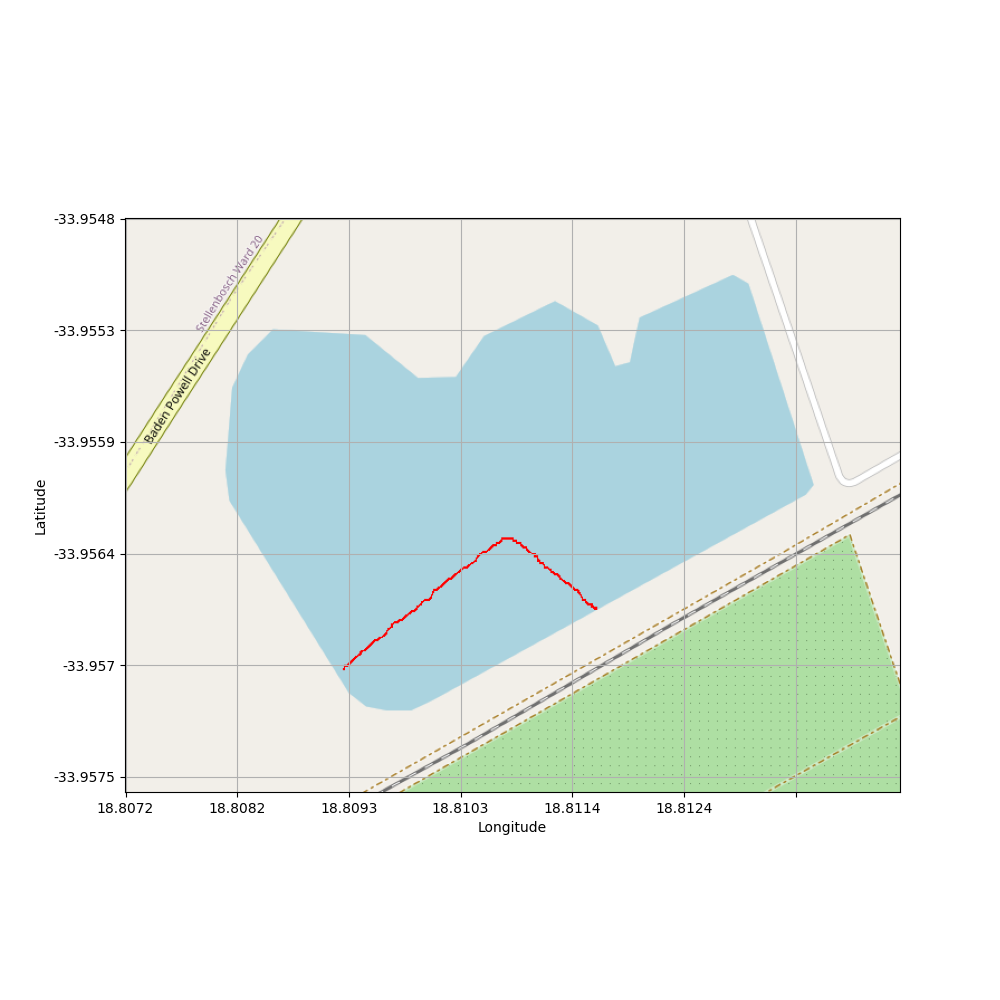
\includegraphics[width=0.8\linewidth]{dam-test-4/dam-test-4.png}
    \caption[Path travelled in first rudder control test]{GPS coordinates of path travelled}
    \label{fig:system-test-2-path}
\end{figure}

The actual and reference heading values logged throughout the test are shown in Fig.\ref{subfig:system-2-headig}. The error signal that was generated for the rudder controller is shown in 
Fig.\ref{subfig:system-2-error}. The change in heading of the vessel corresponds to a spike with an approximate maximum value of $80^{\circ}$ in the error signal. It should be noted that 
even though the absolute value of the error signal is capable of being larger than $60^{\circ}$, a check is done in software to keep the PWM value within its limits - which correspond to 
$\pm 60^{\circ}$. 

It can be seen that the rudder controller tracked the reference signal sufficiently throughout the duration of the test, even when an approximate step change 
occurred. The vessel is therefore capable of navigating between multiple waypoints situated outside of the vessels no-sail zone.

\begin{figure}[h!]
    \centering
    \begin{subfigure}{=0.75\linewidth}
        \centering
        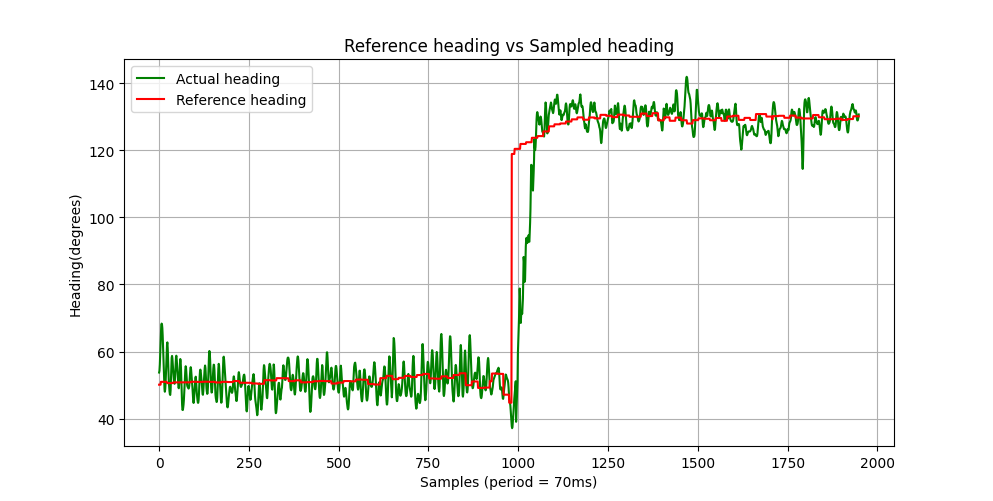
\includegraphics[width=1\linewidth]{dam-test-4/heading.png}
        \caption{Actual and reference heading}
        \label{subfig:system-2-heading}
    \end{subfigure}

    \begin{subfigure}{=0.75\linewidth}
        \centering
        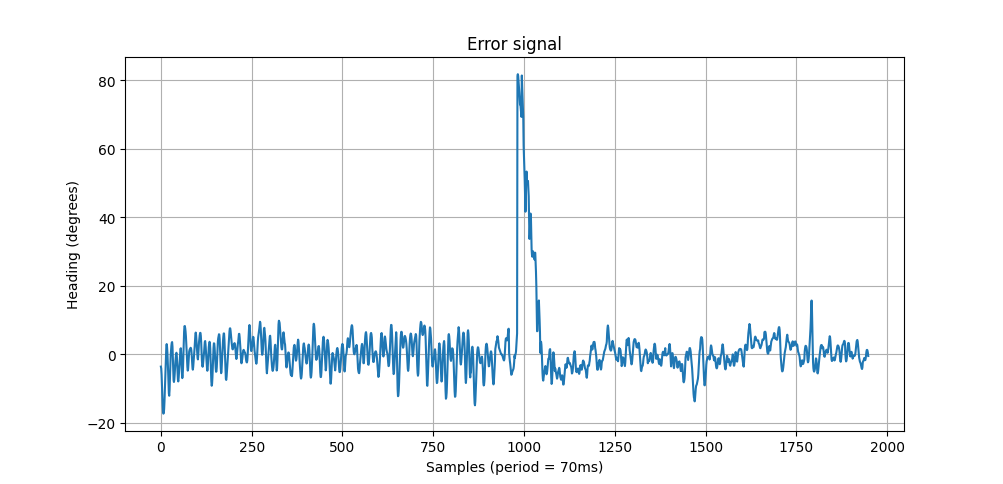
\includegraphics[width=1\linewidth]{dam-test-4/error-sig.png}
        \caption{Error signal}
        \label{subfig:system-2-error}
    \end{subfigure}

    \begin{subfigure}{=0.75\linewidth}
        \centering
        \includegraphics[width=1\linewidth]{dam-test-4/wind.png}
        \caption{Apparent wind}
        \label{subfig:system-2-wind}
    \end{subfigure}

    \caption[Second system test on water]{Second system test on water}
    \label{fig:system-2-water}
\end{figure}

%Must include apparent wind readings as well as sail position here